% !TeX spellcheck = cs_CZ
\begin{mdframed}{Barevné ponožky}{exam006}
  V zásuvce jsou ponožky tří barev. Červené (\textbf{Č}), zelené (\textbf{Z}) a modré (\textbf{M}).
  Je jich tam od každé barvy hodně. Student jde na schůzku a chce si vzít čisté ponožky. Náhle
  zhasne světlo. Student vytáhne potmě dvě ponožky. Jaká je pravděpodobnost, že ponožky budou mít
  stejnou barvu? Vyjmenujme případy, které mohou při vytažení dvou ponožek nastat: (\textbf{Č+Č}),
  (\textbf{Č+Z}), (\textbf{Z+Č}), (\textbf{Č+M}), (\textbf{M+Č}), (\textbf{Z+Z}), (\textbf{Z+M}),
  (\textbf{M+Z}), (\textbf{M+M}). Je tedy \(n = 9\). Příznivé situace jsou tří, (\textbf{Č+Č}),
  (\textbf{Z+Z}), (\textbf{M+M}). Pravděpodobnost je tedy 1/3. (Převzato z
  \cite[s.~200]{Musilova2009MA1}) 

  {\centering
  \captionsetup{type=figure} 
  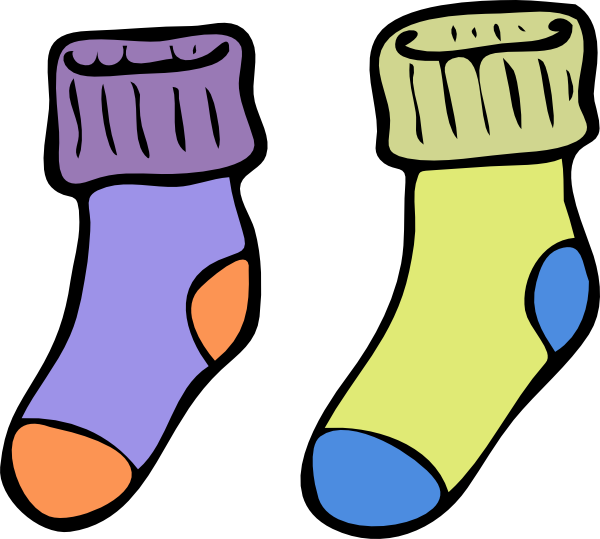
\includegraphics[width=0.2\linewidth]{mai_fig065}
  \captionof{figure}{Ilustace k příkladu \ref{mai:exam006}}
  \label{mai:fig065}
  \par}
\end{mathexam}  